\svnidlong
{$HeadURL$}
{$LastChangedDate$}
{$LastChangedRevision$}
{$LastChangedBy$}
\svnid{$Id$}

%As described in Section~\ref{sec:monojet_scalar}, a model with a scalar/pseudoscalar particle 
%mediating the DM-SM interactions is one of the simplest UV completions of our EFT models.  
With the MFV assumption, the top and possibly bottom
quark can play a primary role in the phenomenology.
The model predicts not only
the monojet process described in Section~\ref{sec:monojet_scalar}, but also production of dark matter
in association with top (or bottom) pairs, as illustrated in Fig.~\ref{fig:TTbarPhi}. 
Dedicated searches including jets from heavy flavor quarks in the final state
can be designed for this production mechanism. Another class of simplified models,  
which includes a Dark Matter interpretation among many others, and yields a single
top quark in the final state, is detailed in Appendix~\ref{sec:singletop}. 

\begin{figure}[h!]
\centering
  \unitlength=0.005\textwidth
  \begin{feynmandiagram}[modelTTbarMET]
    \fmfleft{i1,i2}
    \fmfright{o1,o4,o5,o3}
    \fmf{gluon}{i1,v1}
    \fmf{gluon}{i2,v2}
    \fmf{fermion}{o1,v1,v3,v2,o3}
    \fmf{scalar}{v3,v4}
    \fmf{fermion}{o5,v4,o4}
    \fmf{phantom,tension=0,label={$\phi/a$}}{v3,v4}    
    \fmflabel{\Large $g$}{i1}
    \fmflabel{\Large $g$}{i2}
    \fmflabel{\Large $t (b)$}{o1}
    \fmflabel{\Large $\bar t (\bar b)$}{o3}
    \fmflabel{\Large $\chi$}{o4}
    \fmflabel{\Large $\bar \chi$}{o5}    
  \end{feynmandiagram}
%\caption[][\baselineskip]{Representative Feynman
\caption{Representative Feynman
diagram showing the pair production of dark matter particles in
association with $t\bar t$ (or $b\bar b$).}
\label{fig:TTbarPhi}
\setfloatalignment{t}
\end{figure}



%one of the most simple UV complete extension of the effective field theory approach is the addition of a scalar mediator between DM and SM.
%A gauge singlet mediator can have tree-level interactions with a singlet DM particle that is either a Dirac or Majorana fermion, or DM that is a scalar itself. The spin-$0$ mediator can either be a real or complex scalar; a complex scalar contains both scalar and pseudoscalar particles, whereas the real field only contains the scalar particle.
%In this document we consider only two of the possible choices for this simplified model: one where the interaction with the SM is mediated by a real scalar, and the second where we consider only a light pseudoscalar, assuming that the associated scalar is decoupled from the low-energy spectrum. The kinematics of the two cases is sufficiently different to suggest that further investigation of the complex scalar case is needed but left for future studies. 

%%CD: this sentence really belongs elsewhere: MG does not have the gluon loop
%Couplings to the SM fermions can be arranged by mixing with the SM Higgs. Such models have interesting connections with Higgs physics, and can be viewed as generalizations of the Higgs portal to DM. The most general scalar mediator models will have renormalizable interactions between the SM Higgs and the new scalar $\phi$ or pseudoscalar $a$, as well as $\phi/a$ interactions with electroweak gauge bosons. Such interactions are model dependent, often subject to constraints from electroweak precision tests, and would suggest specialized searches which cannot be generalized to a broad class of models (unlike, for instance, the $\met+\textrm{jets}$ searches). As a result, for this class of minimal simplified models with spin-$0$ mediators, we will focus primarily on couplings to fermions and loop-induced couplings to gluons. Possible couplings to the electroweak sector may also lead to interesting DM phenomenology that can be studied in the context of Higgs Portal DM.

%\subsection{Model and assumption for fermionic DM}

%Minimal Flavor Violation (MFV) implies that scalar couplings to fermions will be proportional to the fermion mass.  However, they can differ for up- and down-type quarks and for charged leptons. 

%Following the assumption that DM is a fermion $\chi$, which couples to the SM only through a scalar $\phi$ or pseudoscalar $a$, the most general tree-level Lagrangians compatible with the MFV assumption are~\cite{Cotta:2013jna,Abdullah:2014lla}:
% \begin{eqnarray}
%{\cal L}_{{\rm fermion},\phi} & = & {\cal L}_{\rm SM}+i\bar{\chi} \slashed{\partial} \chi + m_\chi \bar{\chi}\chi + \left| \partial_\mu \phi \right|^2+\frac{1}{2}m_\phi^2 \phi^2 + \nonumber \\ 
%& &  g_\chi \phi \bar{\chi}\chi+ \frac{\phi}{\sqrt{2}} \sum_i \left(g_u y_i^u \bar{u}_i u_i+g_d y_i^d \bar{d}_i d_i+g_\ell y_i^\ell \bar{\ell}_i \ell_i\right)\, , \label{eq:scalarlag} \\
%{\cal L}_{{\rm fermion},a} & = & {\cal L}_{\rm SM}+i\bar{\chi} \slashed{\partial} \chi + m_\chi \bar{\chi}\chi + \left| \partial_\mu a \right|^2+\frac{1}{2}m_a^2 a^2 + \nonumber \\
%& &  ig_\chi a \bar{\chi}\gamma_5\chi+ \frac{i a}{\sqrt{2}}\sum_i  \left(g_u y_i^u \bar{u}_i \gamma_5 u_i+g_d y_i^d \bar{d}_i \gamma_5 d_i+g_\ell y_i^\ell   \bar{\ell}_i \gamma_5 \ell_i\right) \,. \label{eq:pseudoscalarlag}
%\end{eqnarray}
%Here the sums run over the all SM generations; the Yukawa couplings $y_i^f$ are normalized to $y_i^f = \sqrt{2}m_i^f/v$ where $v \simeq 246 \, {\rm GeV}$ represents the Higgs vacuum expectation value (VEV). We parameterize the DM-mediator coupling as $g_\chi$, without any additional Yukawa structure between the mediator and the dark sector.

%The most general Lagrangians including new scalars or pseudoscalars will have a potential containing interactions with the SM Higgs field $h$. As already stated we only choose a minimal set of interactions that do not include interactions with the Higgs field. Given this simplification, the minimal set of parameters under consideration is
% \bea
%  \left\{ m_\chi,~ m_{\phi/a},~ g_\chi,~ g_u,~ g_d,~ g_\ell \right\} \,.
% \eea
%The simplest choice of couplings, known as Minimal Simplified Dark Matter model (MSDM) \textbf{[TODO: add references]}, is $g_u = g_d = g_\ell$, which is realized in singlet scalar extensions of the SM. 

%Extending the SM Higgs sector to a two Higgs doublet model implies more complex couplings such as  $g_u = \cot \beta$ and $g_d = g_e = \tan \beta$ where $\tan \beta$ denotes the ratio of VEVs of the two Higgs doublets.  The case $g_u \neq  g_d \neq g_\ell$ requires more additional scalars with potentially large masses, and it is not covered here: for simplicity, we assume universal SM-mediator couplings $g_v = g_u = g_d = g_\ell$ in the remainder of this work. 
 
%The expected signal of DM pair production depends on the production rate defined by the dark matter mass $m_\chi$, mediator $m_{\phi/a}$, on the couplings $g_i$ and on the branching ratio defined by the total decay width of the mediator $\phi/a$. We calculate the minimum possible width (assuming only decays into the dark matter and the Standard Model fermions) that is consistent with a given value of $g_\chi g_q$, and assuming all couplings to SM particles equal $\gq = g_u = g_d = g_\ell$. These are given by Eq.~\myeq{eq:width} \cite{Buckley:2014fba}. 

%\begin{equation} \label{eq:width}
%\begin{split}
%\Gamma_{\phi,a}  = & \sum_f N_c \frac{y_f^2 g_q^2 m_{\phi,a}}{16 \pi} \left(1-\frac{4 m_f^2}{m_{\phi,a}^2}\right)^{3/2}
%                   + \frac{g_\chi^2 m_{\phi,a}}{8 \pi} \left(1-\frac{4 m_\chi^2}{m_{\phi,a}^2}\right)^{3/2}\\
%                 & + \frac{\alpha_s^2 y_t^2 g_q^2 m_{\phi,a}^3}{32 \pi^3 v^2} \left| f_{\phi,a}\left(\tfrac{4m_t^2}{m_{\phi,a}^2} \right)\right|^2
%\end{split}
%\end{equation}

%where

%\bea \label{eq:fphifa}
%f_\phi (\tau) = \tau \left [ 1+ (1-\tau) \arctan^2 \left ( \frac{1}{\sqrt{\tau-1}} \right ) \right ]  \,, \qquad 
%f_a (\tau) =  \tau \arctan^2 \left ( \frac{1}{\sqrt{\tau-1}} \right ) \,. 
%\eea

%The first term in each width corresponds to the decay into SM fermions, and the sum runs over all kinematically available fermions, $N_c = 3$ for quarks and $N_c = 1$ for leptons. The second term is the decay into DM, assuming that is kinematically allowed. The factor of two between the decay into SM  fermions and into DM  is a result of our choice of normalization of the Yukawa couplings due to spin dependencies. The last two terms correspond to decay into gluons.  Since we have assumed that $\gq = g_u = g_d = g_\ell$, we have included in the partial decay widths $\Gamma (\phi/a \to gg)$ only the contributions stemming from top loops, which provide the by far largest corrections given that $y_t \gg y_b$~etc. At the loop level the mediators can decay not only to gluons but also to pairs of photons and other final states if kinematically accessible. However the decay rates $\Gamma (\phi/a \to gg)$ are always larger than the other loop-induced partial widths, and in consequence the total decay widths $\Gamma_{\phi/a}$ are well approximated by the corresponding sum of the individual partial decay widths involving DM, fermion or gluon pairs. It should be noted that if  $m_{\phi/a} > 2m_t$ the total widths of $\phi/a$ will typically be dominated by the partial widths to top quarks.

%\section{Specific models involving $b-$ quarks in the final state}

In some theoretically motivated scenario (e.g. for high $tan\beta$ in 2HDM in the pMSSM), 
spin-0 mediators might couple more strongly to down generation quarks.
This assumption motivates the study of final states involving $b$-quarks 
as a complementary search to the $t\bar
t$+DM models presented in the previous section, to directly probe the $b-$ quark coupling. 
In addition to the example illustrated in Fig.~\ref{fig:TTbarPhi}, an example of such a model can be found in Ref.~\cite{Buckley:2014fba}.
Note that, because of the kinematics features of $b$ quark production relative
to heavy $t$ quark production, a $b\bar b$+DM final state may only yield one
experimentally visible $b$ quark, leading to a mono-$b$ signature in a model that conserves $b$ flavor.

%\subsubsection{Parameter scan}

%As discussed in Sec.~\ref{subsec:MonojetLikeModels}, the MFV and universal coupling assumptions for spin-$0$ 
%mediators lead to quark mass dependent Yukawa couplings and therefore dominant couplings to top quarks.

The parameter scan for the dedicated $t\bar{t}$+\MET{} searches has been studied in detail to target the production 
mechanism of DM associated to heavy flavor quarks, still sharing many details of the scan for the scalar model with a gluon radiation 
The benchmark points scanning the model parameters have been selected to ensure that the kinematic features of the 
parameter space are sufficiently represented. Detailed studies were performed to identify points in the \mdm, 
$m_{\phi,a}$, $\gDM$, $\gq$ (and $\Gamma_{\phi,a}$) parameter space that differ significantly from each other 
in terms of expected detector acceptance. Because missing transverse momentum is the key observable for searches, the 
mediator $p_{T}$ spectra is taken to represent the main kinematics of a model. Another consideration in determining the set 
of benchmarks is to focus on the parameter space where we expect the searches to be sensitive during the 2015 LHC run. 
Based on a projected integrated luminosity of $30\,{\rm fb}^{-1}$ expected for 2015, we disregard model points with a 
cross section times branching ratio smaller than $0.1\,{\rm fb}$, corresponding to a minimum of one expected event 
assuming a conservative 0.1\% signal efficiency. 

The kinematics is most dependent on the masses \mdm and $m_{\phi,a}$. Figure~\ref{fig:scanPhi} 
and~\ref{fig:scanPhiPseudo} show typical dependencies for scalar and pseudoscalar couplings respectively.
Typically, the mediator $p_T$ spectra broadens with larger $m_{\phi,a}$. 
The kinematics are also different between on-shell ($\mMed>2\mdm$) and off-shell ($\mMed<2\mdm$) mediators as discussed in Section~\ref{sec:monojet_scalar}. 
Furthermore, the kinematic differences in \MET{} spectrum between scalar and pseudoscalar are larger for light mediator 
masses with respect to heavier mediators. It is therefore important to  
benchmark points covering on-shell and off-shell mediators with sufficient granularity, including the
transition region between on-shell and off-shell mediators. %, as inFig.~\ref{fig:scanPhidiag}. 

\begin{figure}[!ht]
  \begin{center}
    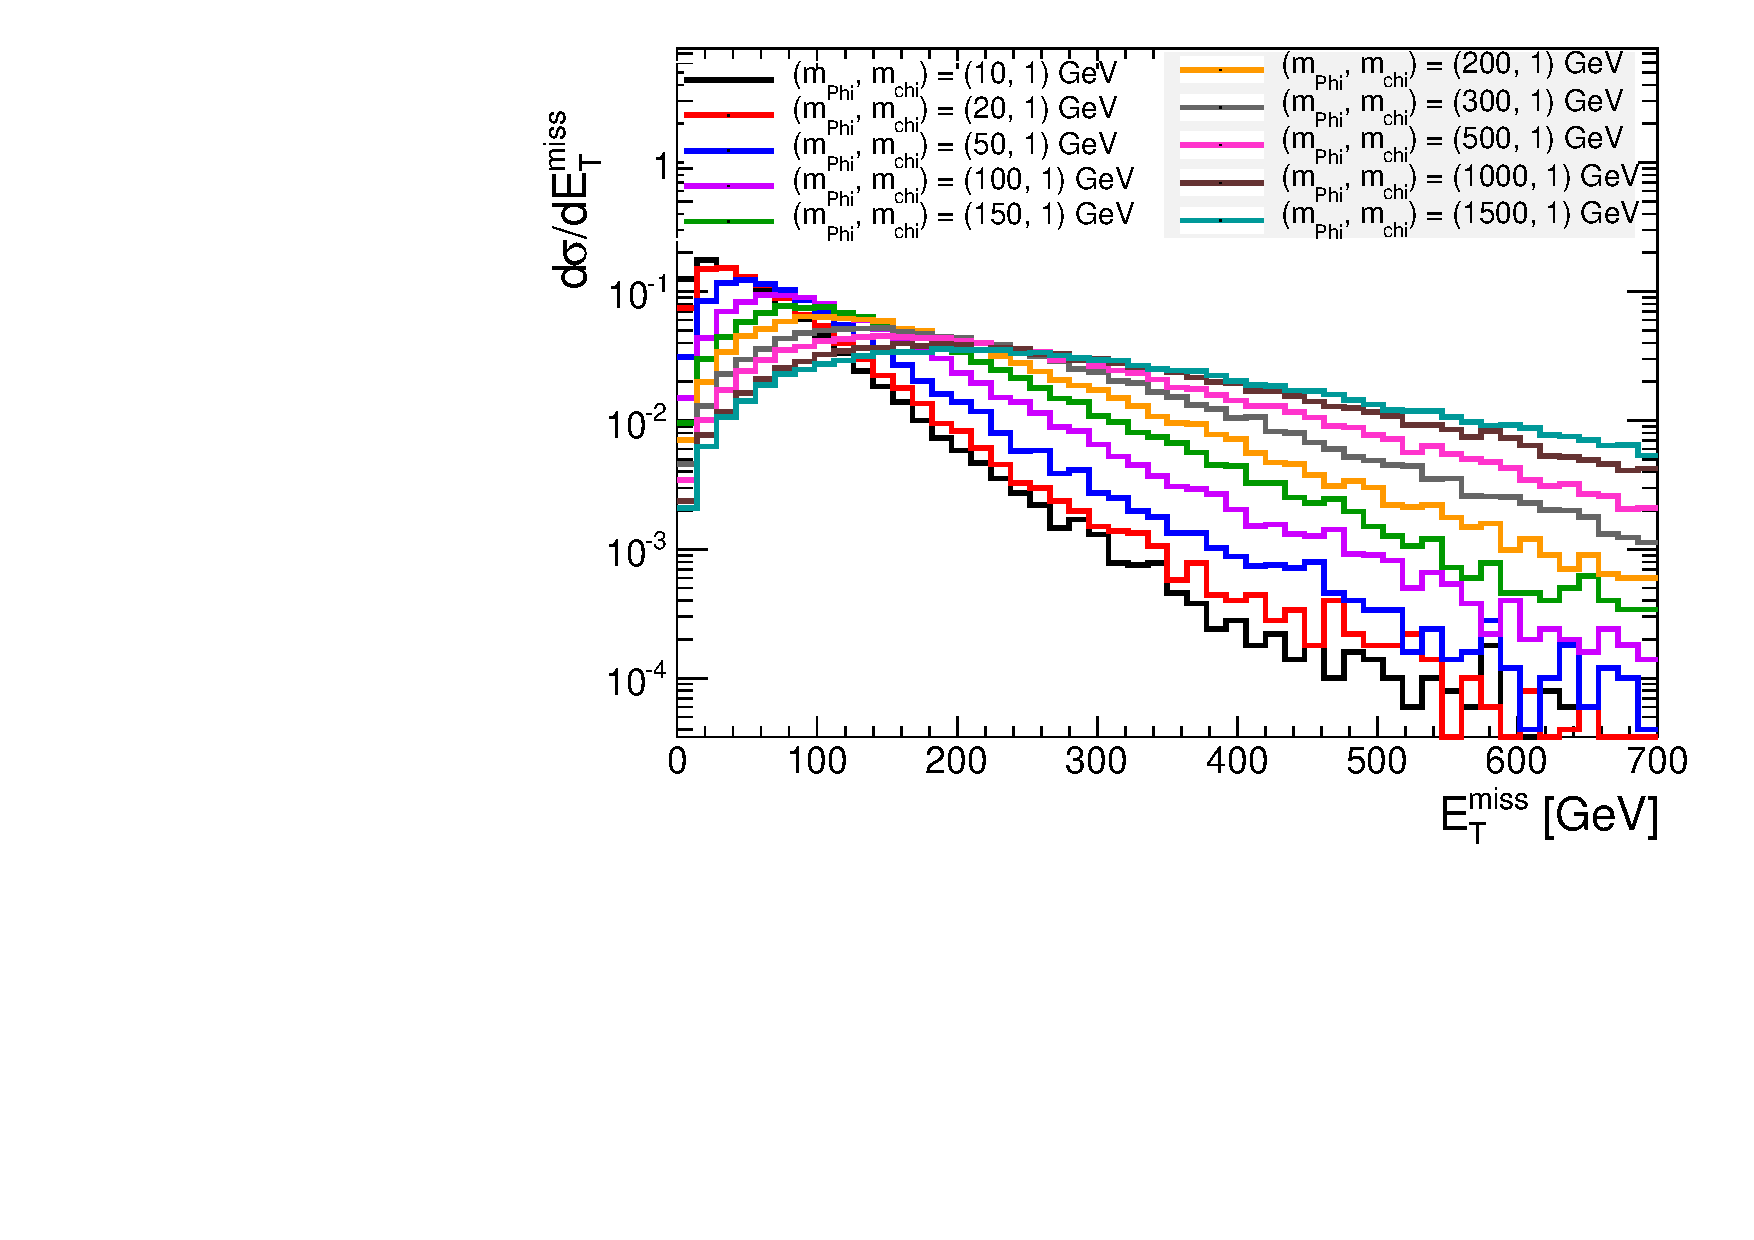
\includegraphics[width=0.7\textwidth]{figures/ttbar/MEt_chi1.pdf}
    \caption{\label{fig:scanPhi} Example of the dependence of the kinematics on the scalar mediator mass. The Dark Matter mass is fixed to be \mdm=$1 {\rm GeV}$.}
\end{center}
\end{figure}


\begin{figure}[!ht]
  \begin{center}
    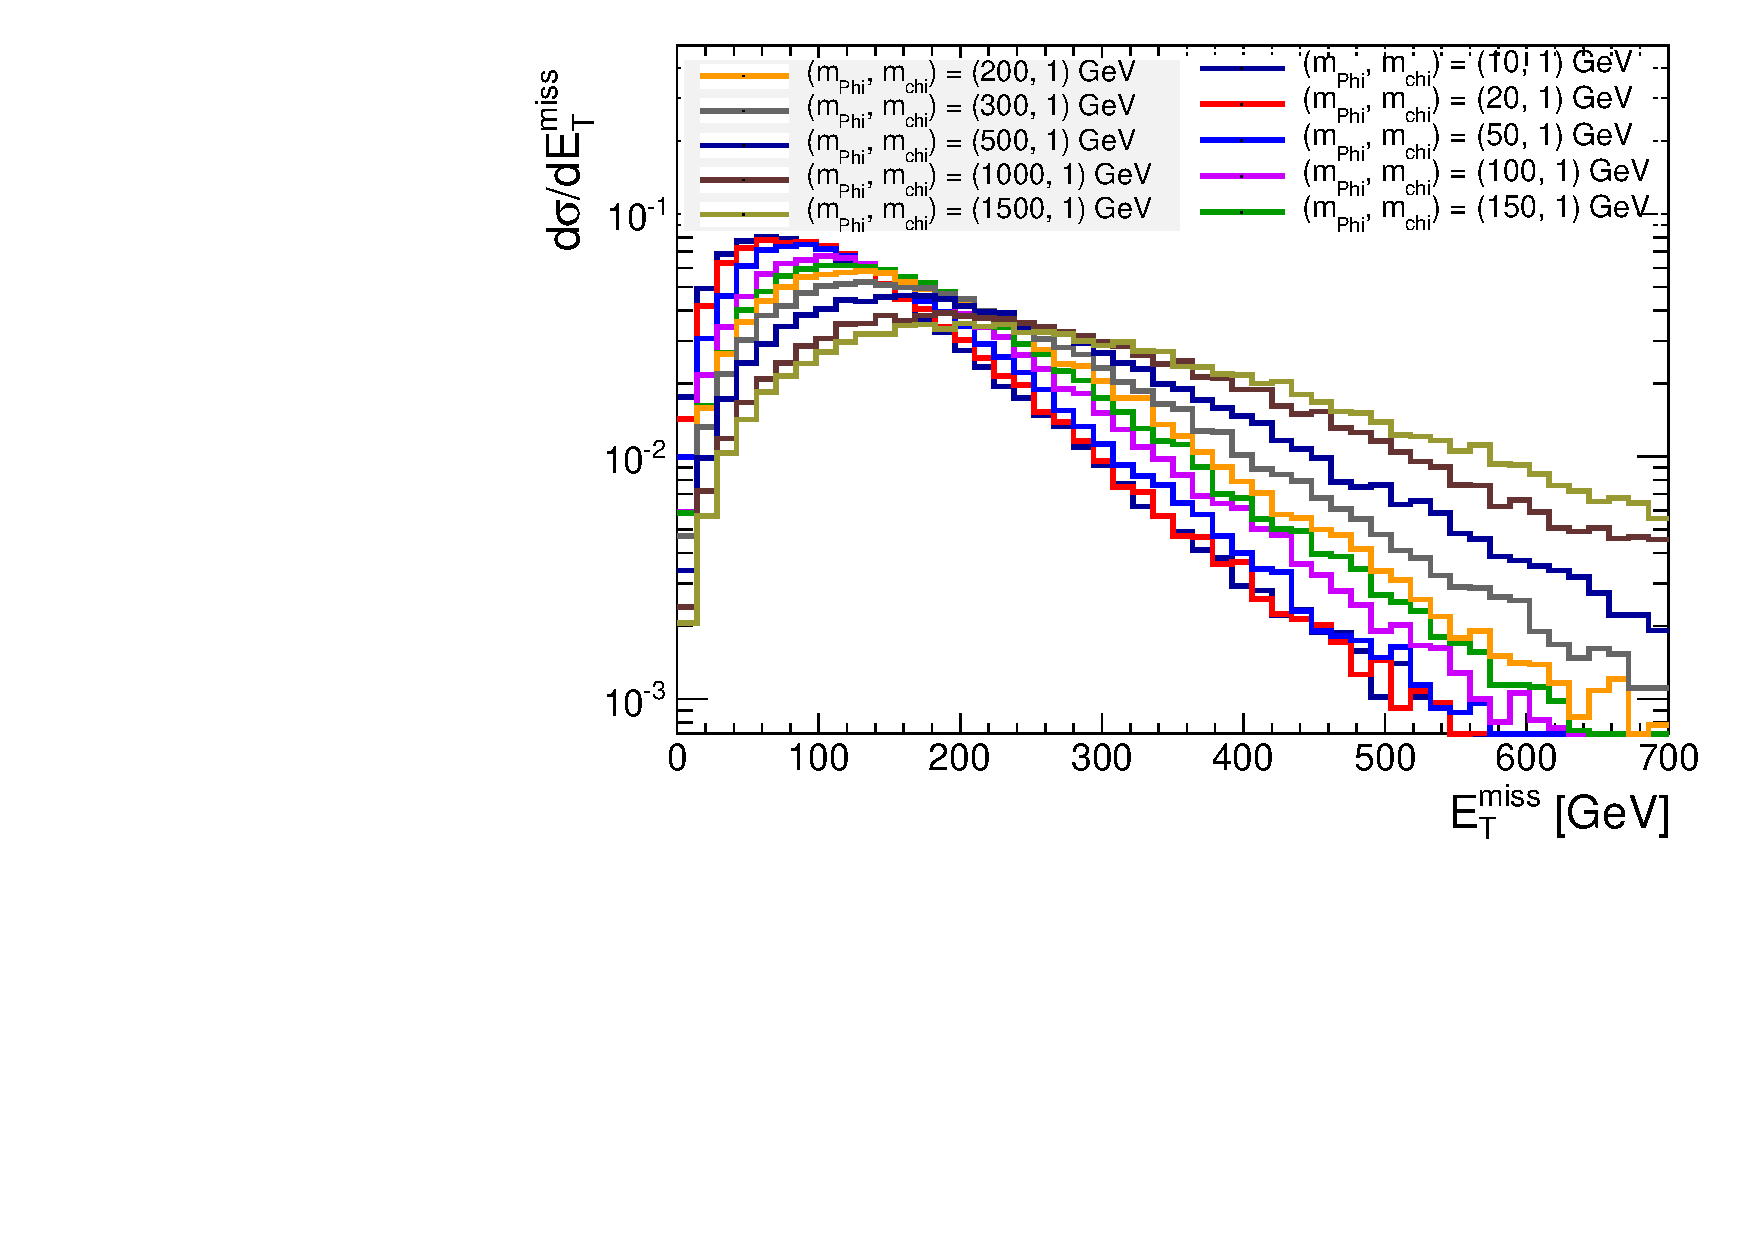
\includegraphics[width=0.7\textwidth]{figures/ttbar/MEt_chi1_pseudo.pdf}
    \caption{\label{fig:scanPhiPseudo} Example of the dependence of the kinematics on the pseudoscalar mediator mass. The Dark Matter mass is fixed to be \mdm=$1 {\rm GeV}$.
    }
\end{center}
\end{figure}

%\begin{figure}[!ht]
%  \begin{center}
%    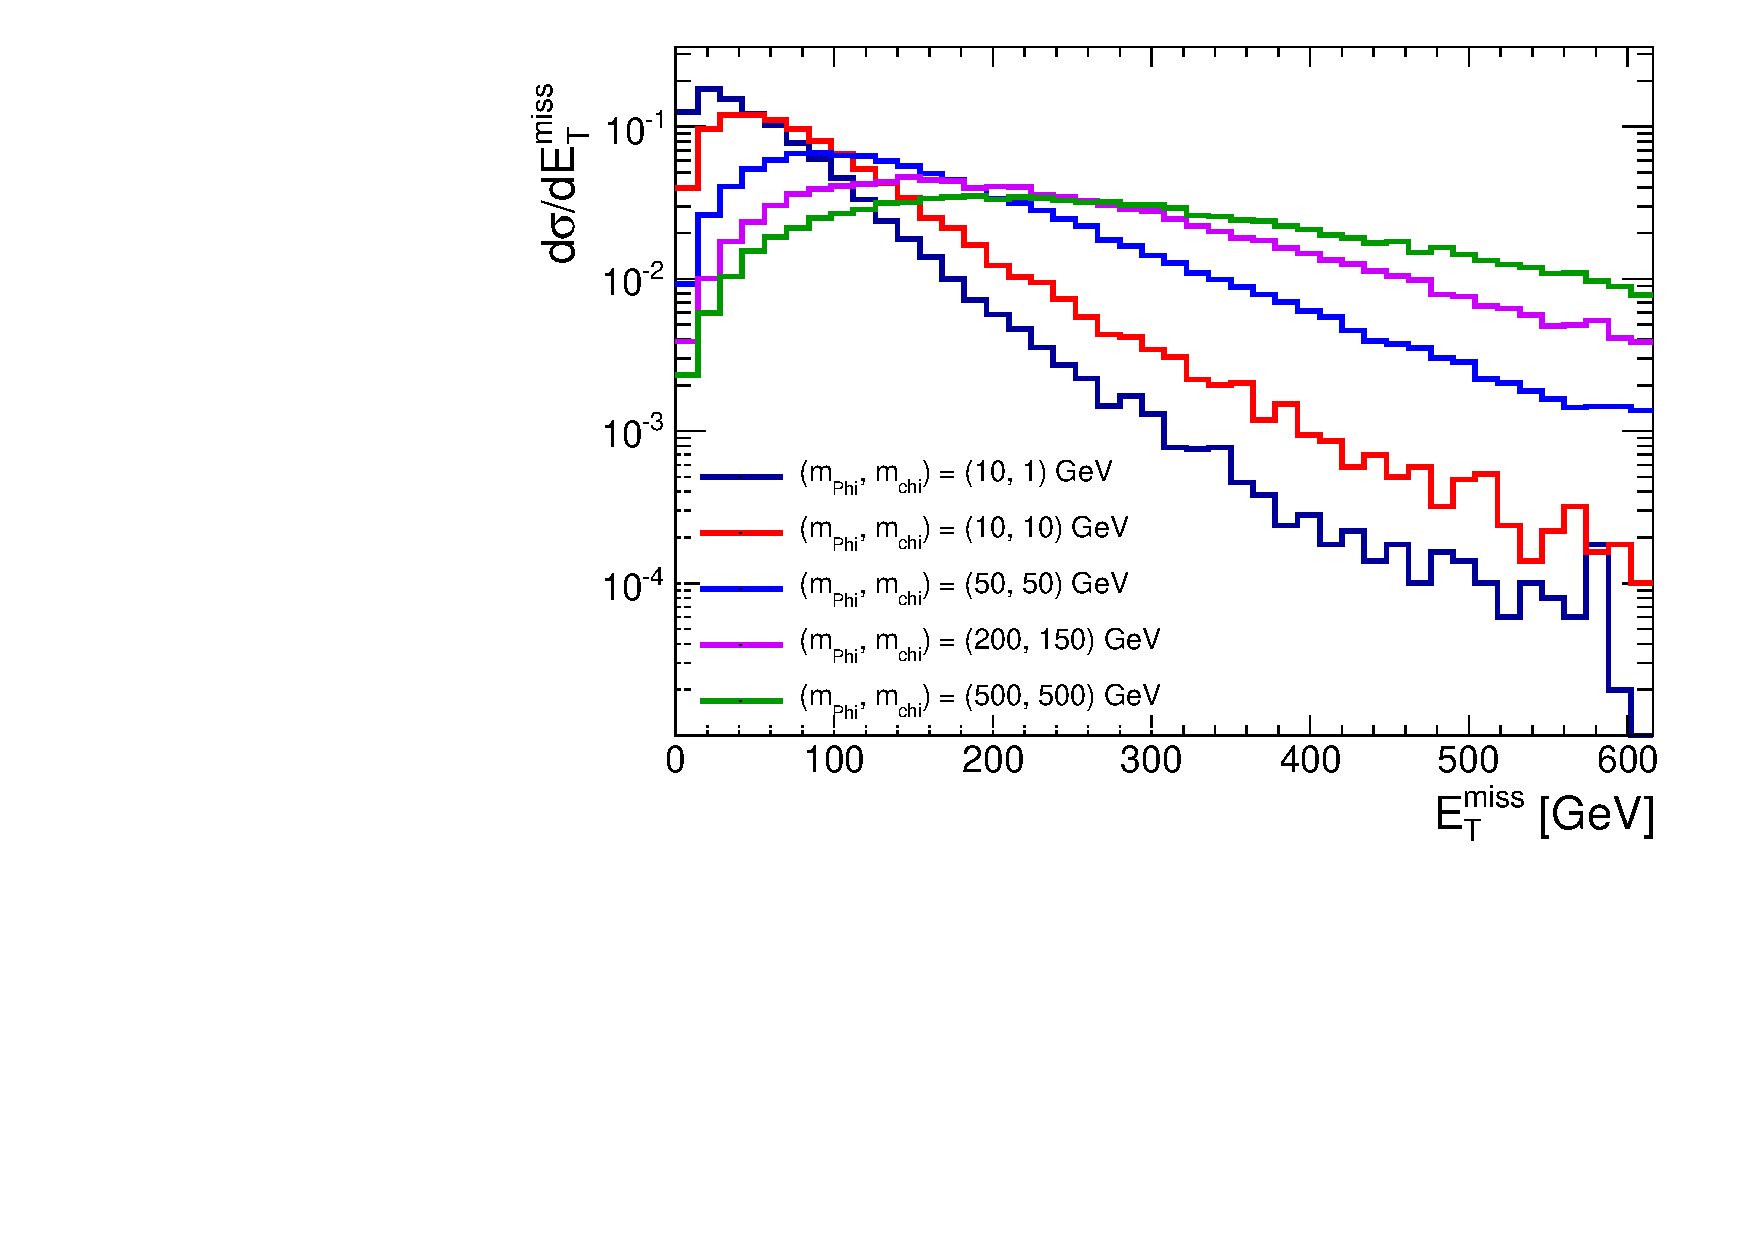
\includegraphics[width=0.7\textwidth]{figures/ttbar/MEt_diagonal_scan.pdf}
%    \caption{\label{fig:scanPhidiag} Example of the dependence of the kinematic for points of the grid proposed in Tab.~\ref{sec:monojet_scalar} close to the $m_{\phi,a} \sim 2m_\chi$ limit.
%    }
%\end{center}
%\end{figure}

Typically only weak dependencies on width or equivalently couplings are observed (see Fig~\ref{fig:widthsmallscan}), except for large mediator masses of $\sim 1.5\,{\rm TeV}$ or for very small couplings of $\sim 10^{-2}$. These regimes where width effects are significant have production cross sections that are too small to be relevant for $30\,{\rm fb}^{-1}$ and are not considered here. However, with the full Run-2 dataset, such models may be within reach. The weak dependence on the typical width values can be understood as the parton distribution function are the dominant effect on mediator production. As shown in Section~\ref{sub:parameter_scan_monojet}, for couplings $\sim O(1)$ the width is large enough that the $p_T$ of the mediator is determined mainly by the PDF.

\begin{figure}[!ht]
  \begin{center}
    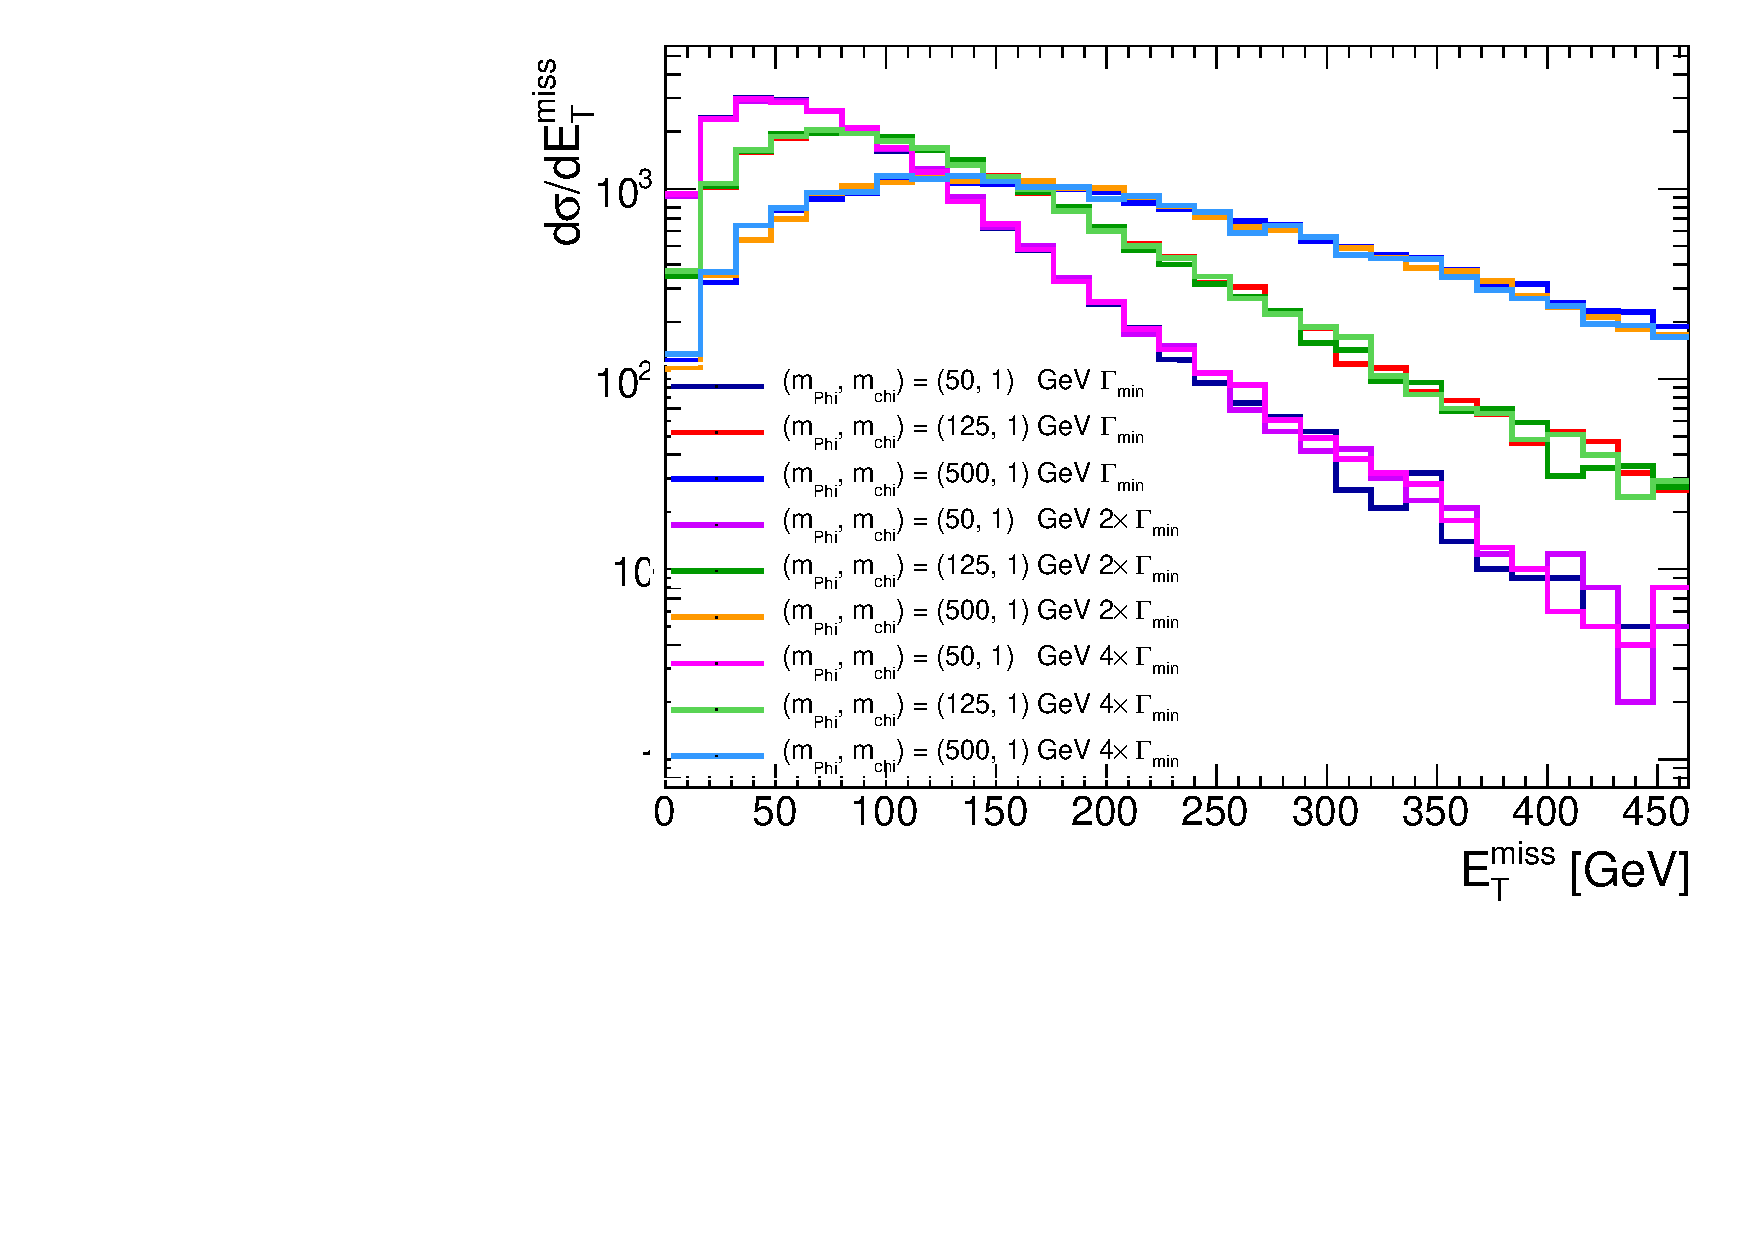
\includegraphics[width=0.7\textwidth]{figures/ttbar/MEt_smallwidth.pdf}
    \caption{\label{fig:widthsmallscan} Study of the dependence of kinematics on the width of a scalar mediator. The width is increased up to four times the minimal width for each mediator and dark matter mass combination. 
    }
\end{center}
\end{figure}

Another case where the width can impact the kinematics is when $m_{\phi,a}$ is slightly larger than $2m_\chi$. Here, the width determines the relative contribution between on-shell and off-shell mediators. An example is given in Fig.~\ref{fig:widthlargescan}. As the minimal width choice pursued in this document is the most conservative one, this effect can be neglected in order to reduce the number of benchmark points to be generated. 

%In our recommendations we propose to use for simplicity the minimal width, as this is represents the most conservative choice to interpret the LHC results. 

\begin{figure}[!ht]
  \begin{center}
    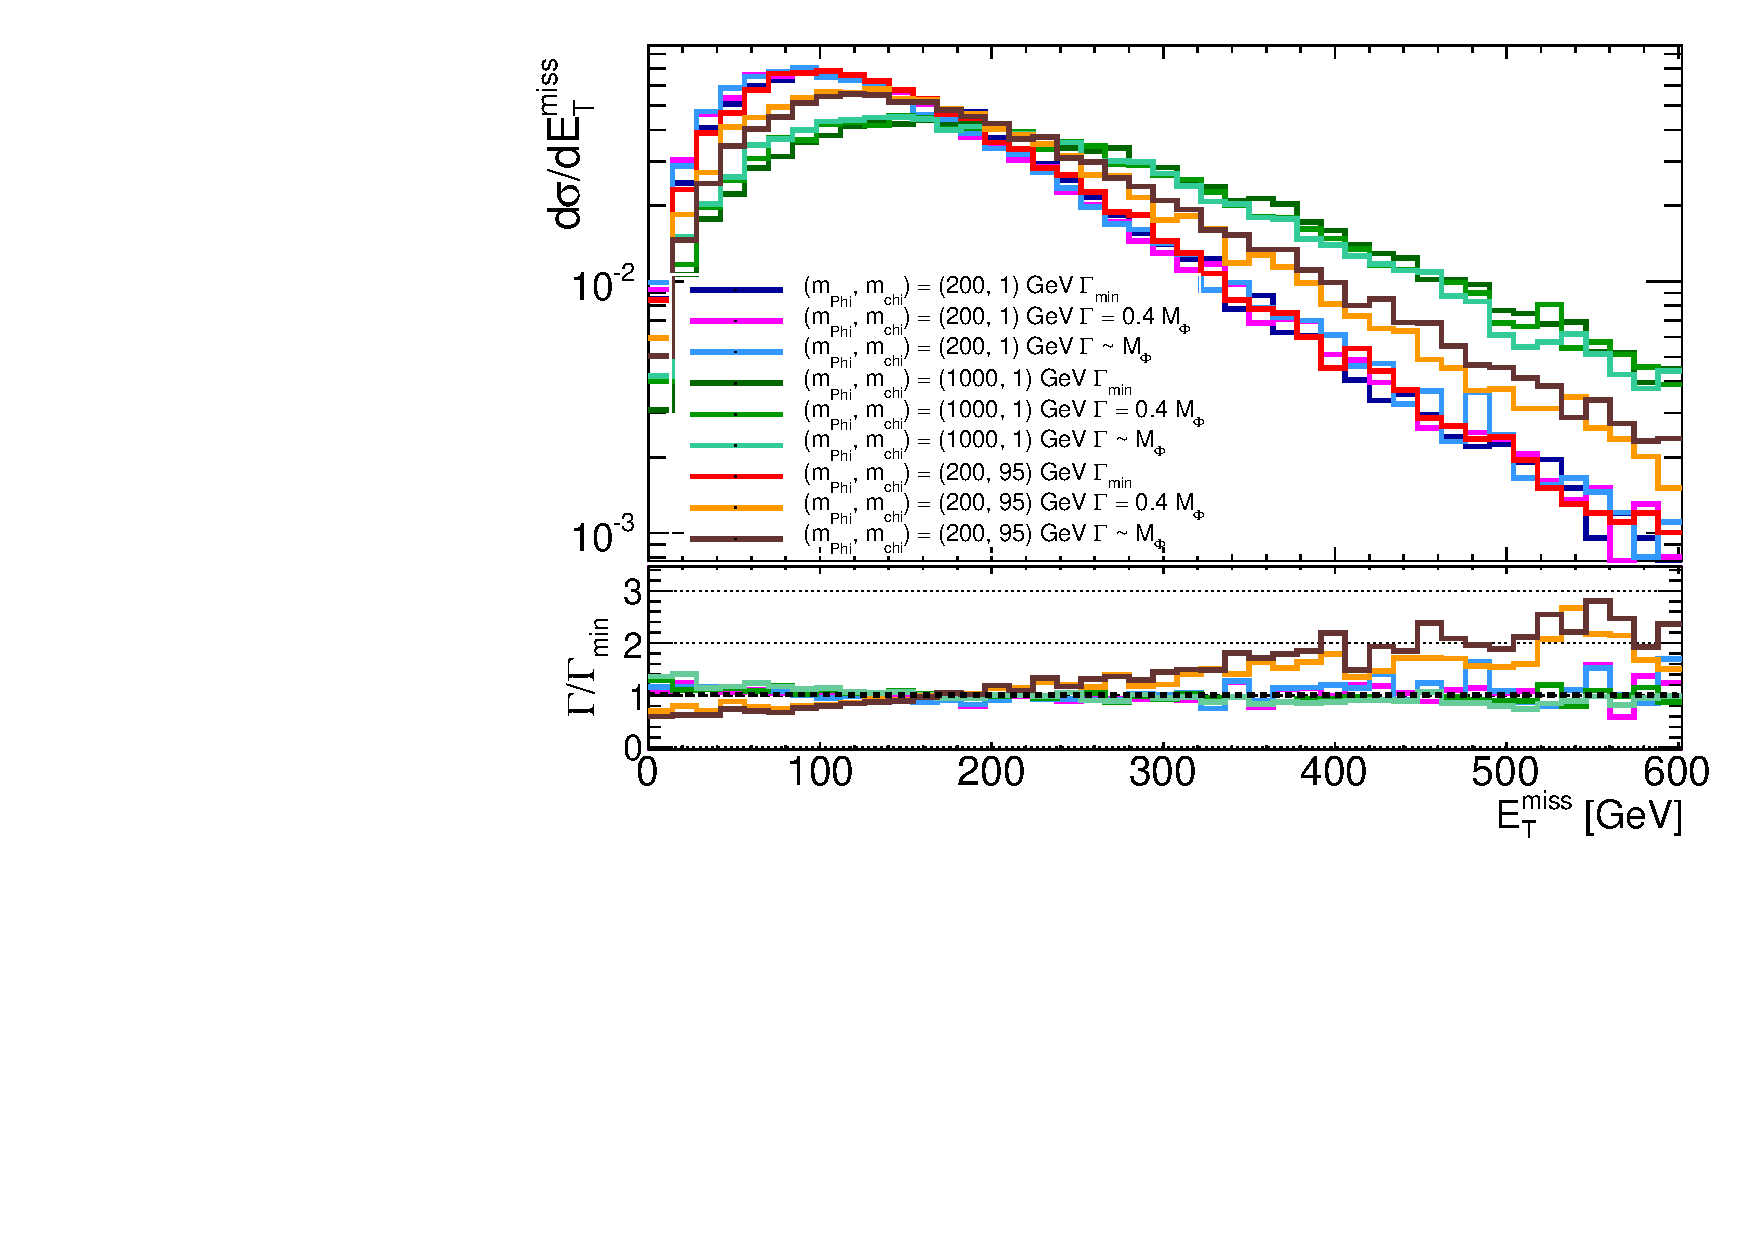
\includegraphics[width=0.7\textwidth]{figures/ttbar/ScalarWidth.pdf}
    \vspace{2mm}
    \caption{\label{fig:widthlargescan} Dependence of the kinematics on the width of a scalar mediator. The width is increased up to the mediator mass. Choices of mediator and dark matter masses such that $m_{\phi,a}$ is slightly larger than $2m_\chi$ is the only case that shows a sizeable variation of the kinematics as a function of the width.  
    }
\end{center}
\end{figure}

The points for the parameter scan chosen for this model are listed in Table~\ref{tab:mDMmMedScan_SP}, chosen
to be harmonized with those for other analyses employing the same scalar model as benchmark. 
Based on the sensitivity considerations above, DM masses are only simulated up to 500 GeV (but the 5 TeV mediator point is retained)
leading to a total of 24 benchmark points. However for these searches we recommend to generate scalar and pseudoscalar
models separately, as the kinematics differs due to the different coupling of the mediator to the final state top quarks in the two cases,
as shown in Figs.~\ref{fig:scanPhi} and ~\ref{fig:scanPhiPseudo}.

Similar studies were performed in the $b \bar b$ case. It was found that they 
show the same weak dependence of the kinematics of the event on the mediator width.
The same benchmark parameters of the $t\bar t$ case could then be chosen.

%%
%[24/05/15 23:48:07] Caterina Doglioni: the plots are made with 5F, while we recommend 4F scheme
%[24/05/15 23:49:04] Caterina Doglioni: even though the relevant parameters do not change 
%(there are some plots due in the appendix for that, albeit with limited statistics), she doesn’t want to put them in 
%and wouldn’t be able to remake them with the right flavor scheme.

% Plots for bbar, if they make it
% Removing these plots as they won't make it last-minute. 
%\Todo{[TODO: The following figures are placeholders for now and will be added later].  If these are supporting material for the MC generation, put in the appendix}.
%
%\begin{figure}
%    \vbox{\hfill}
%    \caption{\label{fig:bbscanPhi} Example of the dependence of the kinematics on the scalar mediator mass. 
%    	The Dark Matter mass is fixed to be $1 {\rm GeV}$.}
%\end{figure}
%
%\begin{figure}[!ht]
%    \vbox{\hfill}
%    \caption{\label{fig:bbscanPhiPseudo} Example of the dependence of the kinematics on the pseudoscalar mediator mass. 
%    	The Dark Matter mass is fixed to be $1 {\rm GeV}$.}
%\end{figure}


%\newthought{Implementation}
%There are some subtleties to the Monte Carlo simulation relevant for
%this case that are discussed in Appendix~\ref{app:MonojetLikeModels_Appendix}.

%In addition to the considerations discussed in the preceding subsections, very light DM fermions are included ($\mdm=10\,{\rm GeV}$) 
%as this is a region where colliders have a complementary sensitivity to current direct detection experiments. 
% 
% \begin{table}[!ht]
% \centering
% \begin{tabular}{| l | r |}
% \hline
% \multicolumn{1}{|c|}{\mdm (${\rm GeV}$)} & \multicolumn{1}{c|}{$m_{\phi,a}$ (${\rm GeV}$)} \\
% \hline
%  $1$    & $10$, $20$, $50$, $100$, $150$, $200$, $300$, $500$, $1000$, $1500$  \\
%  $10$   & $10$, $20$, $50$, $100$, $150$, $200$, $300$, $500$, $1000$, $1500$  \\
%  $50$   &             $50$, $100$, $150$, $200$, $300$, $500$, $1000$, $1500$  \\
%  $150$  &                          $150$, $200$, $300$, $500$, $1000$, $1500$  \\
%  $500$  &                                               $500$, $1000$, $1500$  \\
% \hline
% \end{tabular}
% \caption{Simplified model benchmarks for $t\bar{t}$+DM production via spin-0 mediators decaying to Dirac DM fermions taking the minimum width presciption for $g_v = \gDM = 1$.}
% \label{tab:ttdm_benchmarks}
% \end{table}
% 
